\documentclass[acmsmall,authorversion]{acmart}
\usepackage{graphicx} % Required for inserting images
\usepackage{amsthm}
\newtheorem{definition}{Definition}
\bibliographystyle{ACM-Reference-Format}


\title{AI at the Crossroads of Science: Foundation Models, Innovation Dynamics, and the Future of Research}
\author{Ana Trisovic ET AL}
\date{February 2024}

\begin{document}

\maketitle

\section{Introduction}

In recent years, foundation models and generative AI have demonstrated remarkable proficiency in a wide range of domains. These advancements encompass a broad spectrum of applications, from language processing to scientific tasks in drug discovery, biology, computational chemistry, and material design, as well as synthetic data generation and simulation. As these trends continue to evolve, our project aims to explore the effect of AI on scientific innovation, methodology, and community by carrying out a comprehensive large-scale analysis of scientific citation and literature. Primarily, we measure the rate of AI innovation, the rate of creating specialized specific-purpose AI by building on existing foundation models, and the rate of model reuse as part of a scientific toolbox for broader research questions. Secondarily, we offer insights into the characteristics of the most widely used foundation models, comparing their utilization based on versatility, accessibility, and performance. This comparison addresses claims that AI is not only transforming science but also creating an uneven playing field, as the most advanced AI technologies become accessible only to a select few with the necessary computing power, expertise, and resources. Our goal is to gain insight into how scientific occupation and methods are changing with AI, the industry-academic dynamics, and the distinction between open-source and proprietary AI models, thus enabling researchers and policymakers to better navigate these evolving dynamics.

\subsection{Foundation models}

Foundation models, primarily recognized for their impact on Natural Language Processing (NLP), represent a broader paradigm shift in artificial intelligence (AI) beyond their initial domain of application~\cite{bommasani2021opportunities}. We adopt the following definition of foundation models:

\begin{definition}
Foundation models are a type of machine learning model that is pretrained on broad data, often using self-supervision, to create adaptable systems for various tasks.
\end{definition}

These models, such as GPT-3, BERT, or DALL-E 2, can be fine-tuned for specific applications with much less labeled data compared to traditional AI techniques. They serve as the basis for various AI applications by leveraging self-supervised learning and transfer learning to apply knowledge across different tasks. Foundation models are designed to produce a wide variety of outputs, such as text, images, or audio generation, and can be used as standalone systems or as a base for other applications. They require vast amounts of data and computational resources for their development and training.

\subsection{Foundation model lifecycle}

We distingush between foundation model \textit{resarch} and \textit{deployment}. Research is demonstrated through theoretical and performance improvements. Model deployment makes a direct impact as it is available for use by researchers, practicioners and general public.

The lifecycle of a foundation model can be broken down into several stages, including:

\begin{enumerate}
    \item Data Collection: Gathering relevant data for training and evaluation.
    \item Training: Using the collected data to train a foundation model. The process adjusts the model's parameters to minimize error and improve its ability to predict or classify new, unseen data.
    \item Adaptation: Modifying the foundation model to perform specific tasks or operate within a particular system. Adaptation makes a general-purpose foundation model applicable to specialized tasks and contexts.
    \item Deployment: Making the adapted model available for use.
\end{enumerate}


\subsection{Industry and Academia}

Foundation model technology draws from extensive research in machine learning, optimization, NLP, and computer vision, contributed by both academia and industry. However, the development of foundation models has largely been the purview of the tech industry, including major companies like Google, Facebook, Microsoft, Huawei, and startups such as OpenAI and AI21 Labs.

The shift towards industry dominance in artificial intelligence (AI) research, particularly in deep learning, is marked by the industry's control over essential resources: computing power, large datasets, and expertise. This control is not only reshaping AI research outcomes, including academic publications and cutting-edge models but also raises concerns for global policymakers about the scarcity of public interest alternatives in AI tools~\cite{ahmed2023growing}.

\subsection{Accessibility and Openness}

\iffalse
Academia has not been able to participate in the fullest way possible due to the loss in accessibility. One of the often overlooked effects of the deep learning revolution was the increase in reproducibility and open science: it increasingly became the norm to publicly release code and datasets, and packages such as TensorFlow [Abadi et al. 2016] and PyTorch [Paszke et al. 2019] made it much easier for people to collaborate and build off of each other’s work. Initiatives like the ML Reproducibility Challenge10 as well as reproducibility checklists adopted by major conferences [Pineau et al. 2020], alongside platforms like CodaLab Worksheets11 helped advance community standards for reproducibility. This resulted in a surge in technological innovation and progress.

Foundation models start to roll back this positive trend. Some models (e.g., GPT-3) are not released at all (only API access to a limited pool of people). Even datasets (e.g., for GPT-2) are not released. While trained models may be available (e.g., BERT), the actual training of foundation models is unavailable to the vast majority of AI researchers, due to the much higher computational cost and the complex engineering requirements.
S
ome meaningful research can still be done by training smaller models within reach of an academic budget, and indeed the surprisingly regularity predicted by scaling laws [Kaplan et al. 2020] make this a viable strategy for cases where the differences due to scale are quantitative (e.g., accuracy goes up). However, due to the emergent nature of these foundation models, some functionalities like in-context learning have only been demonstrated in models of sufficient size, so scale is needed to even ask the right questions.
\fi

\subsection{Foundation Model Transparecy Index}


Foundation Model Transparency Index (FMTI)~\cite{bommasani2023foundation} consists of 100 indicators that comprehensively codify what it means for a foundation model developer to be transparent.

Foundation models are released by different developers using a variety of release strategies (Liang et al, 2022b; Solaiman, 2023)

\iffalse
Every open developer is nearly at least as transparent in terms of aggregate score as the highest-scoring closed developer (OpenAI): Meta and Hugging Face are at least 5 points higher, and Stability AI is within a point of OpenAI. Many closed developers provide products built on top of their flagship foundation model, providing users of their platforms and clients who license their proprietary foundation models with an opportunity to push for transparency. Our findings dispel the belief that closed developers are more likely to be transparent about downstream matters due to their greater control over deployment, while emphasizing that both open and closed developers continue to be extremely opaque in terms of the downstream impact of their foundation models. Foundation models are being developed, deployed, and adopted at a frenetic pace: for this technology to advance the public interest, real change must be made to rectify the fundamental lack of transparency in the ecosystem.
\fi

\section{Methods and Analysis}

The particular challenge of our research lies in detecting nuance in the nature of AI referencing and usage in the scientific literature. For instance, a paper introducing a novel foundation model might reference existing foundation models, but not directly build on those models. In other cases, researchers may directly build on existing models by fine-tuning or transfer learning. The subtle difference in these definitions of reuse presents a challenge in their detection and classification. In order to address this challenge we carry out a transformer-based analysis of research literature and use a combination of techniques including prompt engineering and fine-tuning of large language models. We build on the previous effort on paper citation intent classification and leverage existing models and data benchmarks for citation classification. However, most of the previous efforts have been focused on detecting citation sentiment and position in the paper, rather than detecting reuse nuance. 

Regarding the technical implementation, our starting point is a list of foundation models and their properties, including their size, authors, institute, year of release, performance, and availability, which is manually collected. To understand how these models were used in research, we retrieve all available papers that reference the foundation models through a standard scientific citation via the Semantic Scholar knowledge base and convert them into simple text format. From there, we use large-language models Llama 2, Mistral, and GPT-4 to answer our research questions. In order to evaluate and establish accuracy in reuse nuance detection, we manually created a ground truth data sample, which involved human labelers (undergraduate students) who classified the reuse of the foundation models based on the citation context. Then, we use this sample to fine-tune, train, and test the large-language models to process scientific articles on a large scale. We obtain results using zero-shot and one-shot learning techniques, followed by fine-tuning and prompt engineering in a question-answering pipeline by passing the article content, and question and retrieving a structured answer. In addition to the evaluation with the ground truth sample, we cross-check our results by leveraging existing citation-intent models. Finally, we align the collected citation data with comprehensive information about the models, allowing us to quantify the impact of various types of foundational models in science, including the prevalence of models characterized by higher accessibility, versatility, and complexity. Additionally, we assess the current state of model accessibility, the extent of reuse, and the contributions of both industry and academia in advancing AI.

\subsection{Dataset}

We use a dataset from Epoch as our starting point.

% TODO Anna
% Summary of the Epoch dataset, how it was collected, what it contains, etc.

\section{Results} 

\subsection{About Models}

We look into 1143 foundation models, which include a variety of model modalities, i.e., language, vision, biology, games, multimodal, robotics, and others. Almost half of the models are language models, with vision models being the second most common (16\%). The models included were published from 1950 to 2024, though the majority include models published from 2016 onwards. Most of the models are documented as academic papers or reports, and they received an average of 358 citations. The most cited model papers are vision and language models. The number of parameters for the smallest models is 10, while for the largest model is over 170 trillion parameters. Each model is classified according to the availability of reuse (as fully open-source, permissive license, weights available, API accessible, and unreleased or proprietary). We find that open-source models are significantly more cited compared to other levels of access (for example almost 5 times more cited than models with accessible API, which is the second most common).

\subsubsection{Keyword Analysis}

% TODO Anna 
% keyword analysis of word trends 
% paper vocab in time

\begin{figure}
    \centering
    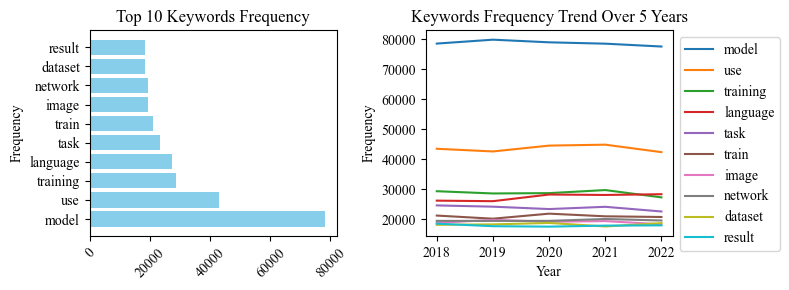
\includegraphics[width=\linewidth]{../figures/keyword_frequencies.png}
    \caption{Keyword trends.}
    \label{fig:keyword-frequencies}
\end{figure}

\subsection{Model Reuse Analysis}

Further, our preliminary results show that the researchers from China and the USA represent a majority of users of the foundation models, with the number of Chinese researchers in some cases even surpassing the US researchers. We find that the reuse domain is mostly computer science, but also medicine, engineering, mathematics, biology, and physics. We observe that the majority of the citations are coming from the same year or the year after the publication of the model paper. The majority of the citations are coming from journal articles, but also from conference papers and books. 

Our preliminary results show that the scientific community mainly uses the foundation models as a tool for their broader research questions. About 25\% of the papers build on the foundation models (though fine-tuning, transfer learning, or other means), and a majority of those introduce the improved model as a stand-alone product rather than part of the methodology for a broader question. These results suggest that there is a large effort in advancing general-purpose foundation models for a specific purpose to carry out specialized tasks that have not previously been augmented by AI.


\bibliography{refs}


\end{document}